%% SORI ↔ SoundPLAN: SoundPLAN 계산 조건(2026-11-17 정리본)에 맞춘 재계산 비교. 단독 컴파일 문서(xelatex 2회)
%% 2026-11-19 개정: SORI 에 반사면–음원 거리 제한(r_refl_source) 추가 → SoundPLAN 반사 규칙 그대로 계산(sp_refl) 결과 반영
%% 2026-11-19 오후 개정: 교통량을 SoundPLAN 입력값(방향별 승용·Trucks1, 사가정로 전 구간)으로 바꿔 다시 계산(sp_refl_1119), 반사 계산 속도 개선(결과 불변)
%% 수치 출처: 비교통계.csv, 비교통계_구간.csv, 비교통계_구역.csv, 조건간_차이.csv (compare_sp_settings.py)
%% 본 문서는 Claude(Anthropic의 AI)를 활용하여 작성하였음.
\documentclass[10pt,a4paper]{article}
\usepackage[a4paper,top=16mm,bottom=16mm,left=17mm,right=17mm]{geometry}
\usepackage{fontspec}
\usepackage{xetexko}
\IfFontExistsTF{Noto Serif CJK KR}{%
  \setmainfont{Noto Serif CJK KR}\setsansfont{Noto Sans CJK KR}%
  \setmainhangulfont{Noto Serif CJK KR}\setsanshangulfont{Noto Sans CJK KR}%
  \setmonohangulfont{Noto Sans CJK KR}[Scale=0.85]}{%
  \setmainfont{Times New Roman}\setsansfont{Apple SD Gothic Neo}%
  \setmainhangulfont{AppleMyungjo}[AutoFakeBold=2.5]\setsanshangulfont{Apple SD Gothic Neo}%
  \setmonohangulfont{Apple SD Gothic Neo}[Scale=0.85]}
\usepackage{booktabs,tabularx,array,graphicx,xcolor,colortbl}
\usepackage{enumitem,needspace}
\usepackage[hidelinks]{hyperref}
\linespread{1.1}
\setlength{\parindent}{0pt}
\setlength{\parskip}{0.35em}
\setlist{itemsep=0.1em,topsep=0.25em}
\renewcommand{\tablename}{표}
\renewcommand{\figurename}{그림}
\newcolumntype{L}{>{\raggedright\arraybackslash}X}
\newcolumntype{R}{>{\raggedleft\arraybackslash}X}
\newcommand{\f}[1]{\texttt{#1}}
\newcommand{\hl}[1]{\textbf{#1}}
\newcommand{\ok}{\textcolor{green!45!black}{같음}}
\newcommand{\nb}[1]{\textcolor{orange!80!black}{#1}}

\begin{document}

{\sffamily\Large\bfseries SORI와 SoundPLAN 비교 — SoundPLAN 계산 조건에 맞춰 다시 계산}\\[1mm]
{\sffamily 전농사거리 동쪽 사가정로 구간 · SORI v0.9(+ 반사면–음원 거리 제한) · RLS-19 · 2026년 11월 19일}

\vspace{2mm}
\fcolorbox{blue!50!black}{blue!5}{\parbox{\dimexpr\linewidth-2\fboxsep-2\fboxrule}{\small
\textbf{요약.} 「SoundPLAN 계산 조건 정리」(11-17)에 적힌 설정에 SORI를 맞춰 다시 계산했다. 반사면 거리 규칙(수음점에서 200 m, 음원에서 50 m)은
SORI에 새 설정을 추가해 그대로 적용했고, 교통량도 SoundPLAN 입력값(동행 1,046 승용 + 388 Trucks1, 서행 838.2 + 267.9 대/h)을 그대로 넣었다.
\begin{itemize}[leftmargin=1.2em]
\item \hl{도로변은 일치한다.} SoundPLAN 75 dB 이상 199점은 평균 −0.49 dB, SD 0.81 dB, ±2 dB 안 93 \%다. 수음점 P1·P2는 \hl{−0.30, −0.32 dB}다.
\item \hl{건물 뒤는 일치하지 않는다.} 남측 큰 건물 뒤(53점)는 \hl{−6.9 dB}, 북측 건물 뒤(31점)는 −4.3 dB로 SORI가 낮고, 남동쪽 건물 사이 틈(19점)은 +4.5 dB로 높다.
전체 554점은 평균 −1.00 dB, SD 3.17 dB, ±2 dB 안 70 \%다. 교통량을 SoundPLAN 입력값으로 바꾼 영향은 점마다 0.2 dB 이하다.
\item \hl{건물 뒤 결과는 반사 거리 규칙에 크게 좌우된다.} 같은 입력에서 반사 거리 규칙만 바꿔도 남측 건물 뒤가 −4.1 \textasciitilde{} −7.0 dB, 북측 건물 뒤가 +0.5 \textasciitilde{} −4.3 dB로 달라진다.
SoundPLAN 규칙을 문자 그대로 적용한 경우가 가장 낮다. SoundPLAN이 ‘음원에서 50 m’를 실제로 어떻게 판정하는지(도로 구간별인지, 도로 전체 기준인지)가
건물 뒤 비교의 핵심 미확인 사항이다.
\end{itemize}}}

\section*{1. 계산 조건 대조}
SoundPLAN 값은 「SoundPLAN 계산 조건 정리」(2026-11-17)의 설정 화면 값이다. 「이전」은 11-12 비교(\f{sagajeong\_only/r2\_ref})의 설정이다.

{\small
\begin{tabularx}{\linewidth}{@{}p{24mm}p{36mm}p{36mm}L@{}}
\toprule
항목 & SoundPLAN & 이전 SORI(11-12) & 이번 SORI \\
\midrule
기준 & RLS-19 배출·전파 & RLS-19 & \ok \\
반사 차수·손실 & 2차, 0.5 dB/회 & 2차, 0.5 dB & \ok \\
반사 거리 & 반사면: 수음점 200 m 안, 음원 50 m 안 & 반사면: 수음점 100 m 안, 음원: 수음점 200 m 안, 2차 50 m & \ok\ 새 설정 \f{r\_refl\_source: 50}, \f{r\_facade: 200}. 경로의 \hl{모든 반사면}에 적용(해석, 4절 1번) \\
측면 회절 & 없음 & 없음(rls19 방법은 적용 안 함) & \ok \\
회절 상한 & 1000 dB(상한 없음) & 상한 없음(RLS-19 식 15) & \ok \\
도로 분할 & 거리/8, 최소 1 m & 3 m 고정 & \ok\ 1 m(s ≥ 8 m에서 l ≤ s/8) \\
탐색 반경 & 5 km & 300 m & \ok\ 1 km(교통량 있는 음원이 모두 수음점에서 600 m 안 → 5 km와 같은 결과) \\
교통량 & 동행 2차로 각 717(523 + 194), 서행 3차로 각 368.7(279.4 + 89.3) 대/h, 화물차 전부 Trucks1 & 양방향 2,540 대/h, p1 25.83 \%(양방향 공통), 측정점 100 m 밖은 50 : 50 & \ok\ 동행 1,046 + 388, 서행 838.2 + 267.9 대/h, p1 동 27.06 \% · 서 24.22 \%(방향별 화물차 비율, 새 기능), 사가정로 전 구간 같은 값 \\
속도 & 남측 50, 북측 30 km/h & 동행 50, 서행 30 & \ok \\
노면 & 기준 노면(0 dB) & 기준 노면 & \ok \\
다중반사 Drefl & 0 dB & \nb{켬}(최대 0.72 dB) & \ok\ 끔 \\
신호교차로 D\textsubscript{K} & 없음 & \nb{자동 판정 켬}(최대 2.97 dB) & \ok\ 끔 \\
도로 높이·경사 & 지형 높이, 평활 0 m & \nb{차도 평탄화(20 m), 지형 평활 5 m} & \ok\ 지형 그대로, 평활 0(경사 산정 구간 30 m는 그대로) \\
지형·건물 & 등고선·표고점, 층수 × 3 m & 같음 & \ok \\
음원 도로 & 사가정로만, 차로마다 음원선 & 사가정로만, 3 + 2 차로 차로별 & \ok\ (사가정로 범위는 11-12와 같은 구간, x 204,755–205,700) \\
수음점·격자 & M1·M2 1.31 m, 격자 5 m·2 m & 같은 좌표·높이 점 수음점 & \ok \\
격자 보간 & 9 × 9 보간(일부 점은 보간값) & 모든 점 직접 계산 & \nb{맞출 수 없음} \\
\bottomrule
\end{tabularx}}

\section*{2. 결과(SORI − SoundPLAN, 격자 552점 + 수음점 2곳 = 554점)}
SoundPLAN 격자 149점은 수치지도 건물 안이라 제외했다(11-17 정리본 권고와 같음).
들여 쓴 비교 조건은 그 항목만 다르다(반사 거리 비교 세 줄은 이전 교통량으로 계산 — 교통량 영향은 0.2 dB 이하).

{\small
\begin{tabularx}{\linewidth}{@{}Lrrrrrrr@{}}
\toprule
조건 & 평균 & SD & RMSE & ±2 dB & r & P1 (74.09) & P2 (77.30) \\
\midrule
이전(11-12) & −0.31 & 3.32 & 3.33 & 61 \% & 0.93 & 74.18 (+0.09) & 77.22 (−0.08) \\
\rowcolor{blue!6}\hl{SoundPLAN 조건 + 반사 규칙 + 교통량} & \hl{−1.00} & \hl{3.17} & \hl{3.32} & \hl{70 \%} & 0.95 & 73.79 (−0.30) & 76.98 (−0.32) \\
\quad 교통량만 이전 값(11-12 구간·공통 p1) & −1.03 & 3.17 & 3.33 & 69 \% & 0.95 & 73.81 (−0.28) & 76.92 (−0.38) \\
\quad 반사 거리만 SORI 기본(100 · 200 · 50 m) & −0.62 & 3.07 & 3.13 & 70 \% & 0.94 & 73.94 (−0.15) & 76.94 (−0.36) \\
\quad 반사 거리만 넓게(반사면 200 m, 음원 제한 없음) & +0.17 & 2.65 & 2.65 & 72 \% & 0.95 & 74.07 (−0.02) & 77.02 (−0.28) \\
\quad 위 + 지형 평활만 이전대로 & +0.10 & 2.63 & 2.63 & 71 \% & 0.95 & 74.07 (−0.02) & 77.02 (−0.28) \\
\bottomrule
\end{tabularx}}

\needspace{12\baselineskip}
\textbf{SoundPLAN 레벨 구간별}(격자 552점; 평균 / SD, dB)

{\small
\begin{tabularx}{\linewidth}{@{}lrRRRR@{}}
\toprule
SoundPLAN LrD & n & 이전(11-12) & \hl{SoundPLAN 조건(최종)} & 반사 SORI 기본 & 반사 넓게 \\
\midrule
≥ 75 (도로변) & 199 & −0.21 / 1.17 & \hl{−0.49 / 0.81} & −0.47 / 0.82 & −0.42 / 0.82 \\
70–75 & 67 & +0.68 / 1.40 & \hl{−0.04 / 0.95} & +0.07 / 0.94 & +0.23 / 0.94 \\
65–70 & 64 & +1.44 / 1.97 & \hl{+0.36 / 1.45} & +0.56 / 1.49 & +0.96 / 1.47 \\
60–65 (건물 뒤가 많음) & 137 & −2.69 / 4.80 & \hl{−3.16 / 4.29} & −2.84 / 4.41 & −0.99 / 3.60 \\
< 60 & 85 & +1.19 / 3.57 & \hl{−0.51 / 4.69} & +1.16 / 3.75 & +2.79 / 3.28 \\
\bottomrule
\end{tabularx}}

\needspace{12\baselineskip}
\textbf{구역별}(그림 1 차이 지도; 평균 / SD, dB)

{\small
\begin{tabularx}{\linewidth}{@{}lrRRRR@{}}
\toprule
구역 & n & 이전(11-12) & \hl{SoundPLAN 조건(최종)} & 반사 SORI 기본 & 반사 넓게 \\
\midrule
남측 큰 건물 뒤(x 205200–205262, y ≤ 553092) & 53 & −7.12 / 3.47 & \hl{−6.90 / 3.92} & −7.02 / 3.37 & −4.12 / 2.97 \\
북측 건물 뒤(x 205160–205205, y ≥ 553155) & 31 & −1.03 / 1.74 & \hl{−4.26 / 2.19} & −1.31 / 1.75 & +0.50 / 1.74 \\
남동 건물 사이 틈(x ≥ 205285, y 553090–553120) & 19 & +4.33 / 4.09 & \hl{+4.49 / 4.00} & +4.76 / 4.21 & +5.97 / 3.77 \\
서쪽(x < 205160) & 138 & +2.05 / 1.65 & \hl{+0.31 / 1.74} & +0.76 / 1.32 & +1.18 / 1.43 \\
그 밖(도로변 등) & 312 & −0.41 / 1.82 & \hl{−0.60 / 1.70} & −0.41 / 1.76 & +0.07 / 1.81 \\
\bottomrule
\end{tabularx}}

\begin{figure}[h]
\centering
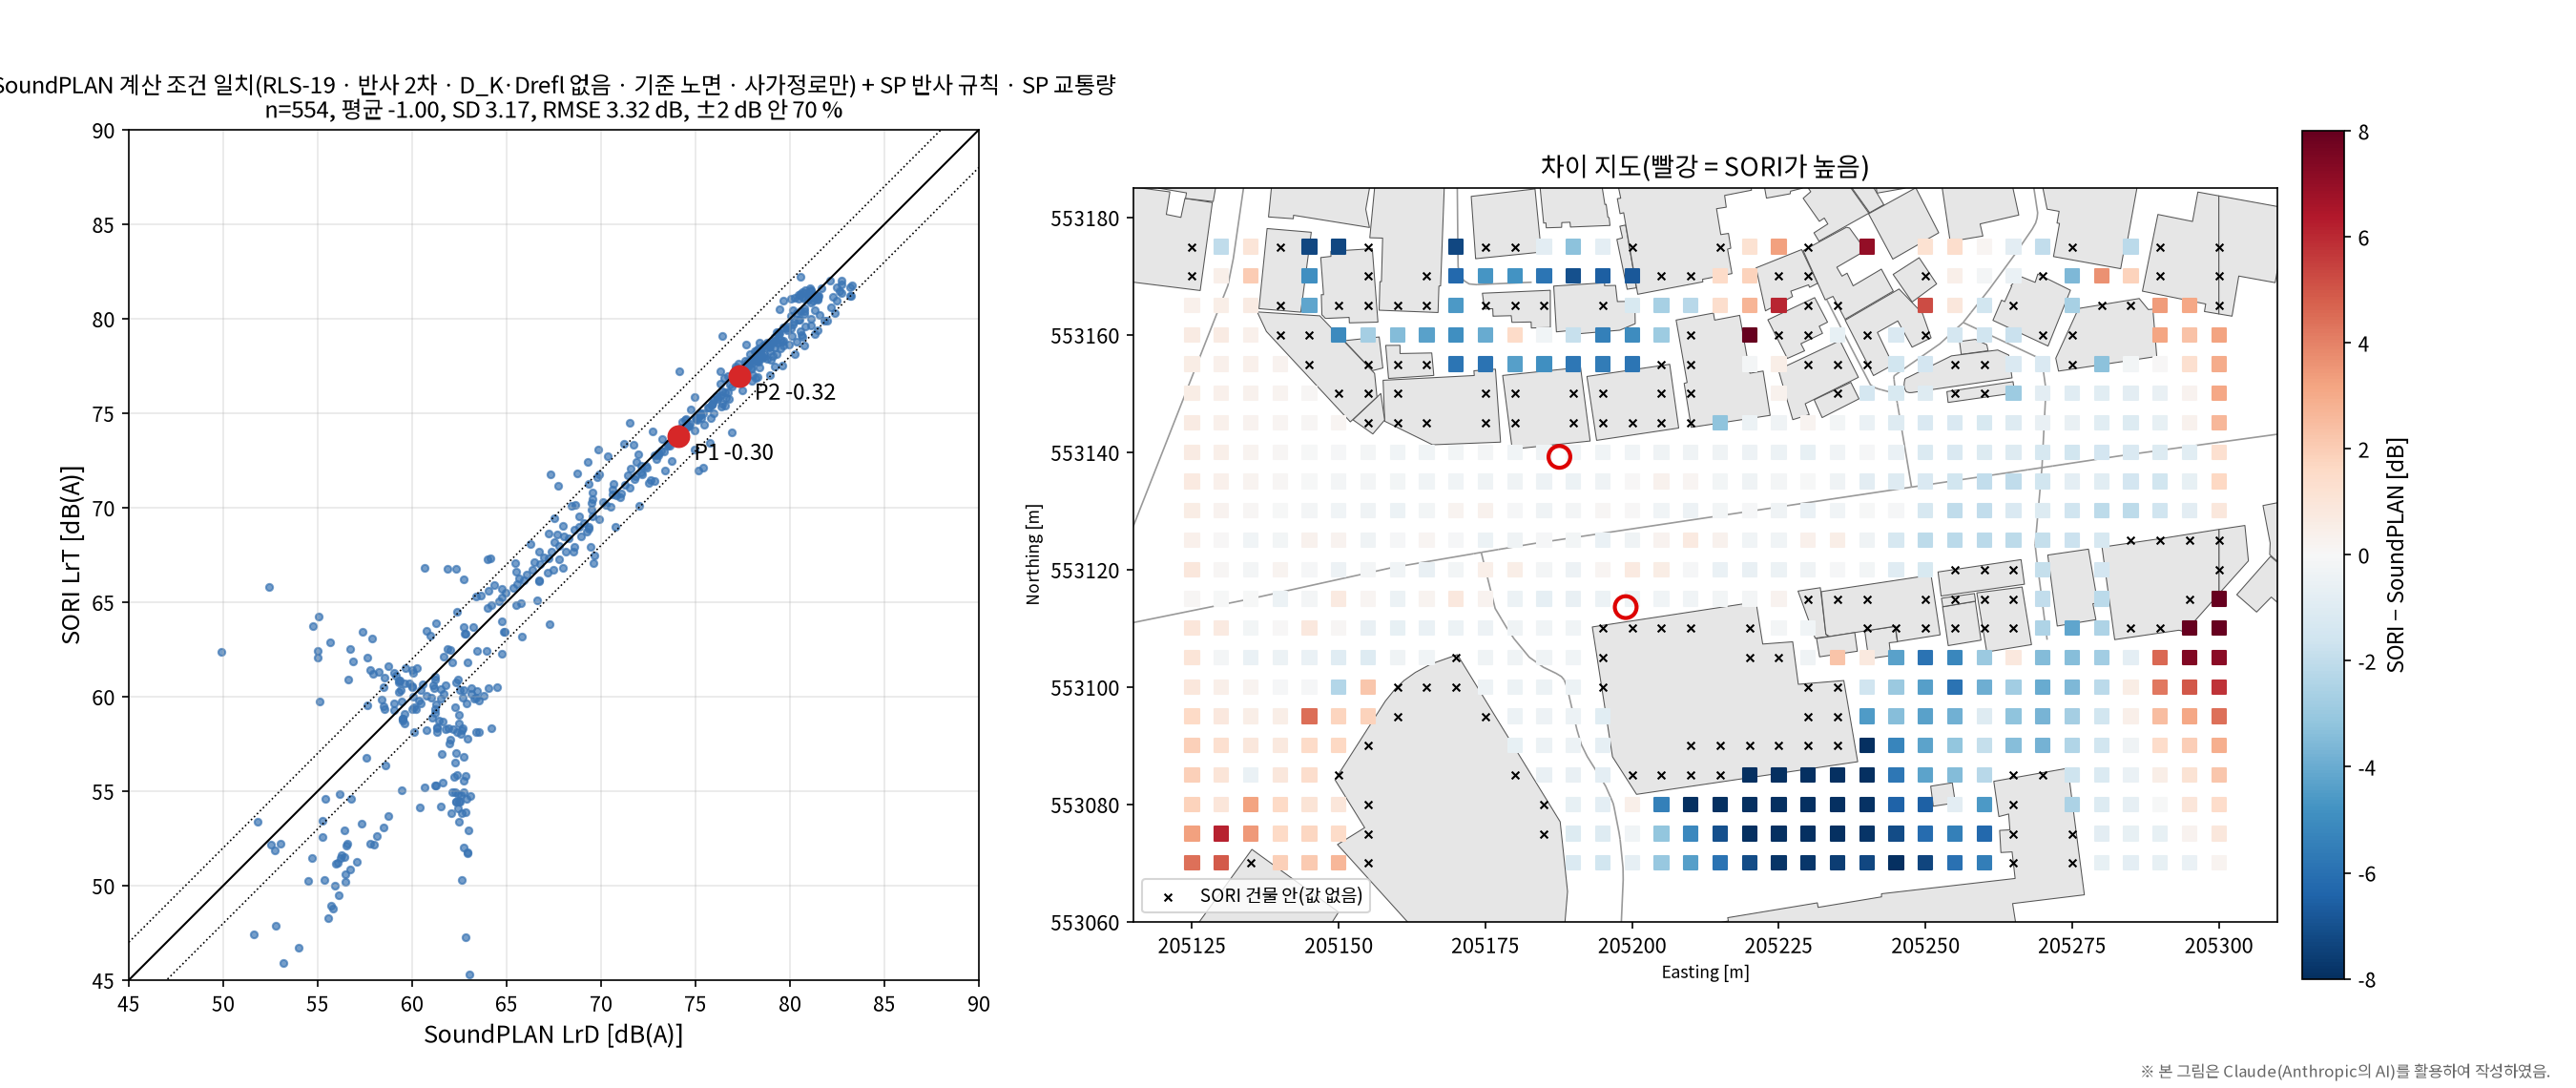
\includegraphics[width=\linewidth]{비교_sp_refl_1119.png}
\caption{SoundPLAN 조건(반사 규칙·교통량 포함). 왼쪽: 점별 비교(점선 ±2 dB). 오른쪽: 차이 지도(빨강 = SORI가 높음, × = SORI 건물 안이라 제외).
반사를 넓게 둔 경우의 그림은 \f{비교\_matched.png}.}
\end{figure}

\section*{3. 무엇이 결과를 바꿨나(같은 554점, SoundPLAN 조건(최종) − 비교 조건)}
{\small
\begin{tabularx}{\linewidth}{@{}Lrrrrrr@{}}
\toprule
비교 조건 & 평균 & |차| 95 \% & 최소 & 최대 & P1 & P2 \\
\midrule
이전(11-12)(D\textsubscript{K}·Drefl·분할·탐색·지형·반사 거리·교통량 모두 다름) & −0.69 & 3.10 & −7.82 & +2.10 & −0.39 & −0.24 \\
교통량만 이전 값 & +0.03 & 0.08 & −0.06 & +0.17 & −0.03 & +0.05 \\
반사 거리 SORI 기본(교통량도 이전 값) & −0.38 & 2.78 & −6.79 & +2.13 & −0.16 & +0.03 \\
반사 거리 넓게(교통량도 이전 값) & −1.17 & 4.71 & −8.88 & +0.06 & −0.28 & −0.05 \\
\bottomrule
\end{tabularx}}

\begin{itemize}
\item \hl{도로변·수음점}: 반사 규칙에 따른 차이가 0.1 \textasciitilde{} 0.3 dB로 작다. D\textsubscript{K}·Drefl 끄기, 분할 1 m, 지형 평활 0으로 바꾼 결과를 합쳐도 이전보다 약 0.3 dB 낮아지는 정도다.
도로변 일치(−0.5 dB, SD 0.8 dB)는 어느 규칙에서나 유지된다.
\item \hl{건물 뒤}: 직접음이 막히는 곳이라 반사음이 레벨을 정한다. 그래서 반사 규칙만 바꿔도 최대 8.9 dB까지 달라진다.
SoundPLAN 규칙을 그대로 쓰면 음원에서 50 m보다 먼 벽의 반사가 모두 빠져 SORI 기본 규칙보다도 더 낮아진다(북측 건물 뒤 −1.3 → −4.3 dB).
\item \hl{교통량}: SoundPLAN 입력값(방향별 화물차 비율, 사가정로 전 구간 같은 방향별 값)으로 바꿔도 점마다 −0.06 \textasciitilde{} +0.17 dB 바뀌는 데 그친다.
\item \hl{지형 평활}: 영향이 작다(평균 +0.07 dB, 95 \% 점이 0.4 dB 안). 따로 맞출 필요는 크지 않다.
\end{itemize}

\section*{4. 남은 차이와 확인할 것}
\begin{enumerate}
\item \hl{‘음원에서 50 m’ 판정 방식(가장 중요).} 이번 계산은 도로를 나눈 \hl{1 m 구간 하나하나}를 음원으로 보고, 경로의 \hl{모든 반사면}이 그 구간에서 50 m 안일 것을 요구했다.
SoundPLAN이 도로 전체(음원선)나 더 긴 분할 구간을 기준으로 거리를 재거나, 첫 반사면에만 이 조건을 적용한다면 반사가 더 많이 들어간다.
그러면 건물 뒤 값은 ‘SoundPLAN 반사 규칙’과 ‘반사 넓게’ 사이에 놓인다. 건물 뒤 차이를 다른 원인으로 돌리기 전에 SoundPLAN 도움말이나 시험 계산
(벽 하나·직선 도로)으로 이 판정 방식을 먼저 확인해야 한다.
\item \hl{어느 규칙에서도 남는 차이.} 남측 큰 건물 뒤는 −4.1 \textasciitilde{} −7.0 dB로 항상 SORI가 낮고, 남동 틈은 +4.4 \textasciitilde{} +6.0 dB로 항상 높다.
반사 규칙만으로는 설명되지 않는 몫이다. 후보는 건물 외곽선·높이 자료 차이(SoundPLAN 격자 149점이 SORI 건물 안), 다중 회절 경로 계산 방식,
SoundPLAN 격자 보간(9 × 9, 40 dB 미만 항상 보간)이다. 모두 확인되지 않았다.
11-17 정리본의 다른 앱 결과(“같은 설정으로 맞춘 뒤에도 건물 뒤 평균 −4.5 dB”)와 방향과 크기가 비슷하다.
\item \hl{사가정로 음원 범위.} SoundPLAN 모델의 사가정로가 어디까지인지는 지도로 확인할 수 없다. SORI는 11-12 비교와 같은 구간(약 1 km)을 썼다.
\item \hl{교통량.} SoundPLAN 입력값(동행 1,434, 서행 1,106.1 대/h)을 그대로 넣었다. 11-17 정리본에 적힌 남측 1,394 / 1,440 대/h는 이 입력과 다른 자료 값이며, 써도 약 0.1 dB 차이다.
\item 격자점은 5 m 간격이라 서로 독립이 아니다. SD·RMSE는 구역별 차이의 크기로 읽는다.
\end{enumerate}

\section*{5. SORI 변경과 다시 계산하는 법}
\begin{tabularx}{\linewidth}{@{}p{30mm}L@{}}
\toprule
SORI 변경 & 새 설정 \f{propagation.reflection.r\_refl\_source}(m). 기본 \f{null} = 사용 안 함이고, 이때 결과는 이전과 비트 단위로 같다.
값을 주면 경로의 모든 반사면이 음원에서 이 거리 안, 수음점에서 \f{r\_facade} 안이어야 한다. 테스트 \f{tests/test\_refl\_source\_limit.py}(평행 두 벽 해석값). 방향별 화물차 비율 열(\f{p1\_day\_fwd} 등, UFID 행, 빈칸 = 공통 p1·p2) 추가, 테스트 \f{tests/test\_dir\_truck\_share.py}. 반사 계산 속도 개선(벽마다 음원 50 m 목록으로 미리 거름, 이전 결과와 비트 단위 일치, 점당 약 1.5 s → 0.08 s). 전체 테스트 388개 통과 \\
설정 & \f{sp\_settings\_1117/sp\_refl\_1119/config.yaml}(최종), \f{sp\_refl}(교통량만 이전), \f{matched}(반사 넓게), \f{r\_default}(반사 SORI 기본), \f{terrain\_old}(지형 평활 이전대로) \\
교통량 & \f{traffic\_soundplan\_1119.csv}(최종, 사가정로 53개 객체), \f{traffic\_sagajeong\_ufid.csv}(이전) \\
앱에서 보기 & \f{03\_전농사거리\_SORI계산/config\_soundplan.yaml}: 같은 조건, 격자는 SoundPLAN 격자점과 같은 위치(552점, 값도 같음) \\
계산 & 각 폴더에서 \f{python -m sori all -c config.yaml}(속도 개선 뒤 조건마다 1 \textasciitilde{} 2분. 격자를 끄고 계산하므로 마지막 그림 단계의 \f{grid\_result.csv} 오류는 무시) \\
비교 & \f{.venv/bin/python -I .../sp\_settings\_1117/compare\_sp\_settings.py} → \f{비교통계*.csv}, \f{조건간\_차이.csv}, \f{비교\_*.png} \\
\bottomrule
\end{tabularx}

\vfill
{\footnotesize\color{gray} ※ 본 문서는 Claude(Anthropic의 AI)를 활용하여 작성하였음. 계산 결과의 검토·검증 책임은 사용자에게 있음.}
\end{document}
